% This is file JFM2esam.tex
% first release v1.0, 20th October 1996
%       release v1.01, 29th October 1996
%       release v1.1, 25th June 1997
%       release v2.0, 27th July 2004
%       release v3.0, 16th July 2014
%   (based on JFMsampl.tex v1.3 for LaTeX2.09)
% Copyright (C) 1996, 1997, 2014 Cambridge University Press

\documentclass{jfm}
\usepackage{graphicx}
\usepackage{epstopdf, epsfig}

% My own packages

\usepackage{ dsfont }
\usepackage{amsmath}

% User-defined commands

\newcommand{\ddt}[1]{\frac{d #1}{dt}}
%\newcommand{\hmone}[1]{\|#1\|_{H^{-1}}}
\newcommand{\hmone}[1]{\|\nabla^{-1} #1\|_{L^{2}}}
\newcommand{\ltwo}[1]{\|#1\|_{L^{2}}}
%\newcommand{\hone}[1]{\|#1\|_{H^{1}}}
\newcommand{\hone}[1]{\| \nabla #1\|_{L^{2}}}
\newcommand{\htwo}[1]{\|#1\|_{H^{2}}}
\newcommand{\sint}[1]{\int_{D} #1 \, d^{d}\mathbf{x}}
\newcommand{\tint}[1]{\int_{0}^{T} #1 \, dt}
\renewcommand{\vec}[1]{\mathbf{#1}}
\newcommand{\linf}[1]{\| #1 \|_{L^{\infty}}}
\newcommand{\tavg}[1]{\langle  #1 \rangle}
\renewcommand{\u}{\mathbf{u}}
%\newcommand{\ppt}[1]{\frac{\partial #1}{\partial t}}
\newcommand{\ppt}[1]{\partial_{t} #1}
\newcommand{\lap}{\Delta }
\newcommand{\invlap}{\Delta^{-1}}
%\newcommand{\lap}{\nabla^{2}}
%\newcommand{\invlap}{\nabla^{-2}}
\newcommand{\pbrac}[1]{\left( #1 \right)}
\newcommand{\sbrac}[1]{\left[ #1 \right]}
\newtheorem{lemma}{Lemma}
\newtheorem{corollary}{Corollary}

\shorttitle{Diffusion effects on optimal mixing and filamentation}
\shortauthor{C. J. Miles and C. R. Doering}

\title{Diffusion effects on optimal mixing and filamentation}

\author{Christopher J. Miles\aff{1,2,3}
  \corresp{\email{cmiless@umich.edu}}
 \and Charles R. Doering\aff{1,2,3}}

\affiliation{\aff{1}Department of Physics, University of Michigan,
Ann Arbor, MI 48104-1040, USA
\aff{2}Department of Mathematics, University of Michigan,
Ann Arbor, MI 48104-1043, USA
\aff{3}Center for the Study of Complex Systems, University of Michigan,
Ann Arbor, MI 48104-1107, USA}

\begin{document}

\maketitle

\begin{abstract}
In this work, we investigate the role of diffusion and its impact on our goals for optimal mixing. We show numerical evidence that diffusion can limit the length scales achievable by a generalized Batchelor length scale [\cite{Batchelor1959a}] for incompressible flows with uniformly bounded energy or rate-of-strain for optimal stirring protocols.  We also show that perfect mixing in finite time is impossible for such constraints by extending the work of \cite{Chi-Cheu1996}.
\end{abstract}

\begin{keywords}
\end{keywords}

\section{Introduction}

Optimal mixing is important to many areas of science and engineering. A question of interest across these domains is ``How can one stir to enhance the rate of mixing?'' We address this question by formulating the problem by considering complete control of an incompressible flow in a periodic domain with mild physical constraints. In particular, we consider a  domain $D=[0,L]^{d}$  where $L$ is the side length and $d$ is the total number of spatial dimensions. All functions defined on $D$ have periodic boundary conditions. Let $\theta(\mathbf{x},t): D \times [0,T] \rightarrow [-1,1]$ be the tracer concentration field that evolves according to the advection-diffusion equation,
\begin{equation}
	\label{eq:PDE_advection}
	\ppt{\theta}+\mathbf{u}\cdot \nabla \theta=\kappa \lap\theta
\end{equation}
where $\kappa$ is the molecular diffusion coefficient and $\mathbf{u}(\mathbf{x},t)$ is an incompressible ($\nabla\cdot \mathbf{u}=0$) velocity field constrained by bounded energy
\begin{equation}
	\label{eq:PDE_energy}
	\linf{\u} \leq U
\end{equation}
or rate-of-strain
\begin{equation}
	\label{eq:PDE_rate-of-strain}
	\linf{\nabla\u} \leq \Gamma.
\end{equation}
We are provided with initial data, $\theta(\mathbf{x},0)=\theta_{0}(\mathbf{x})$. We use the mix-norm throughout to measure homogenization,   $\|\nabla^{-1}\theta(\,\cdot\,,t)\|_{L^{2}}$.
We define the following ratio as a measure of the dominant scalar length scale:
\begin{equation}
\lambda(t)\equiv  \frac{\|\nabla^{-1}\theta(\,\cdot\,,t)\|_{L^{2}}}{\|\theta(\,\cdot\,,t)\|_{L^{2}}}.
\end{equation}

For the energy-bounded flow problem, we non-dimensionalize the system by choosing $L$ as the length scale, $U$ as the velocity scale, and $U/L$ as the time scale. For the enstrophy-bounded flow problem, we choose the same length scale $L$, the velocity scale $L\Gamma $, and  the time scale $1/\Gamma$. Both scaling produce the following form of the advection-diffusion equation,
\begin{equation}
\label{eq:nd_ade}
	\ppt{\theta}+\mathbf{u}\cdot \nabla \theta=\frac{1}{Pe} \lap\theta,
\end{equation}
where $Pe= \frac{UL}{\kappa}$ for the energy-constrained case and  $Pe=  \frac{\Gamma L^2}{\kappa}$ for the enstrophy-constrained case. The constraints on the velocity field become $\linf{\u} \leq 1$ or $\linf{\nabla\u} \leq 1$.

\section{Absolute lower bounds on $\lambda$}

\subsection{Results for $\linf{\nabla \vec{u}} \leq 1$}

Taking the time derivative of $\lambda^2$, we find
%
\begin{equation}
	\ddt{\lambda^2} = \frac{2}{Pe}
		\left[ 
			\frac{\hone{\theta}^2\hmone{\theta}^2}
					{\ltwo{\theta}^4}  
			- 1
		\right]
		+ 2 \frac{\sint{\nabla^{-1}\theta \cdot \nabla\vec{u} \cdot 
							\nabla^{-1}\theta  }}
					  {\ltwo{\theta}^{2}}.
\end{equation}
By H\"older's inequality, we have that
\begin{equation}
\label{eq:length_ineq_rate-of-strain}
	\ddt{\lambda^2} \geq \frac{2}{Pe} \left[ 
			\frac{\hone{\theta}^2\hmone{\theta}^2}
					{\ltwo{\theta}^4}  
			- 1
		\right] - 2  \lambda^2 .
\end{equation}
We can provide a lower bound on $\lambda$ at each instant. By apply Gr\"onwall's inequality and the fact that the bracketed term is greater than or equal to zero, it follows from \eqref{eq:length_ineq_rate-of-strain} that
%
\begin{equation}
\label{eq:exponential_enstrophy}
	\lambda (t) \geq \lambda(0)e^{- t}.
\end{equation}
%
Therefore, perfect mixing in finite time is impossible.

One can show that 
%
\begin{subequations}
\begin{align}
\frac{d}{dt}\left(\frac{\|\nabla\theta\|_{L^{2}}^2}{\|\theta\|_{L^{2}}^2}\right) &= \frac{\|\theta\|_{L^{2}}^2\frac{d}{dt}\|\nabla\theta\|_{L^{2}}^2-\|\nabla\theta\|_{L^{2}}^2\frac{d}{dt}\|\theta\|_{L^{2}}^2}{\|\theta\|_{L^{2}}^4}\\
&= \frac{-2\int \partial_{i}u_{j}\partial_{i}\theta\partial_{j}\theta - \frac{2}{Pe} \|\Delta\theta\|_{L^{2}}^2}{\|\theta\|_{L^{2}}^2}+\frac{2}{Pe}\frac{\|\nabla\theta\|_{L^{2}}^4}{\|\theta\|_{L^{2}}^4} \\
&=-\frac{2}{Pe}\left(\frac{\|\Delta\theta\|_{L^{2}}^2}{\|\theta\|_{L^{2}}^2} - \frac{\|\nabla\theta\|_{L^{2}}^4}{\|\theta\|_{L^{2}}^4} \right) - 2\frac{\sint{\nabla\theta \cdot \nabla\vec{u} \cdot 
							\nabla\theta  }}{\|\theta\|_{L^{2}}^2} 
\\
&\leq 2 \frac{\hone{\theta}^2}{\ltwo{\theta}^2}
\end{align}
\end{subequations}
%
From $\ddt{}\ltwo{\theta}^2 = -\frac{2}{Pe} \hone{\theta}^2$, one finds that 
\begin{equation}
\ltwo{\theta}\geq  \ltwo{\theta_{0}}\exp\left[-\frac{1}{2Pe}\frac{\hone{\theta_{0}}^2}{\ltwo{\theta_{0}}^2}\left(e^{2 t} -1\right)\right]
\end{equation}
Using this with \eqref{eq:exponential_enstrophy}, we find that 
\begin{equation}
\hmone{\theta} \geq  \hmone{\theta_{0}} \exp\left[- t -\frac{1}{2 Pe}\frac{\hone{\theta_{0}}^2}{\ltwo{\theta_{0}}}\left(e^{2 t} -1\right)\right]
\end{equation}

\subsection{Results for $\linf{\u}\leq 1$}
Here we extend the results first introduced by \cite{Chi-Cheu1996}.  It is first useful to express the following quantities as:
%
\begin{eqnarray}
	 \hone{\theta}^2 &=& - 2\sint{\theta \lap \theta} \\
	 							&=& Pe \sint{\theta\left(\ppt{\theta}
	 									-\frac{1}{Pe}\lap \theta\right)} 
	 									-Pe \sint{\theta\left(\ppt{\theta}
	 									+\frac{1}{Pe}\lap \theta\right)} 
\end{eqnarray}
%
\begin{eqnarray}
	\ddt{}\ltwo{\theta}^2 &=& 2\sint{\theta\ppt{\theta}} \\
										 &=&\sint{\theta\left(\ppt{\theta}
	 									-\frac{1}{Pe}\lap \theta\right)} 
										 + \sint{\theta\left(\ppt{\theta}
	 									+\frac{1}{Pe}\lap \theta\right)} 
\end{eqnarray}
%
\begin{eqnarray}
	\ddt{}\hone{\theta}^2 &=& -2\sint{\ppt{\theta}\lap \theta} \\
	 									&=& Pe \sint{\left(\ppt{\theta}
	 									-\frac{1}{Pe}\lap \theta\right)^2} 
	 									-Pe \sint{\left(\ppt{\theta}
	 									+\frac{1}{Pe}\lap \theta\right)^2} .
\end{eqnarray}

We then compute the following derivative:
%
\begin{eqnarray*}
	\ddt{} \pbrac{ \frac{\hone{\theta}^2}{\ltwo{\theta}^2} } 
			&=& \frac{1}{\ltwo{\theta}^4}
			\sbrac{
				\ltwo{\theta}^2\ddt{}\hone{\theta}^2
				-\ddt{}\ltwo{\theta}^2\hone{\theta}^2			
			}\\
			&=& \frac{1}{\ltwo{\theta}^4}
			\sbrac{
				\ltwo{\theta}^2
				\pbrac{
					Pe \sint{\left(\ppt{\theta}
	 									-\frac{1}{Pe}\lap \theta\right)^2} 
 					-Pe\sint{\left(\ppt{\theta}
	 									+\frac{1}{Pe}\lap \theta\right)^2} 
				}
			}\\
		&-&\frac{1}{\ltwo{\theta}^4}
			\sbrac{
				Pe
				\pbrac{
					 \sint{\theta\left(\ppt{\theta}
	 									-\frac{1}{Pe}\lap \theta\right)} 
 				}^2		
 				-
 				Pe
 				\pbrac{
					 \sint{\theta\left(\ppt{\theta}
	 									+\frac{1}{Pe}\lap \theta\right)} 
 				}^2					
			}.
\end{eqnarray*}
%
Using H\"older's inequality and \eqref{eq:PDE_advection}, this simplifies to
%
\begin{eqnarray*}
	\ddt{} \pbrac{ \frac{\hone{\theta}^2}{\ltwo{\theta}^2} } 
			&\leq & \frac{Pe}{\ltwo{\theta}^2}
			\sbrac{
					 \sint{(\vec{u}\cdot \nabla \theta)^2} 
			}.
\end{eqnarray*}
By applying H\"older's inequality again, we have
\begin{equation}
\label{eq:k2growth_energy}
	\ddt{} 
		\pbrac{ 
			\frac{\hone{\theta}^2}{\ltwo{\theta}^2} 
		} 
		\leq  
		Pe
		\frac{\hone{\theta}^2}{\ltwo{\theta}^2} .
\end{equation}
%
Thus, we find that 
%
\begin{equation}
		\frac{\hone{\theta}}{\ltwo{\theta}} 
		\leq  
		\frac{\hone{\theta_0}}{\ltwo{\theta_0}}
		\exp{\pbrac{\frac{Pe}{2} t}}
\end{equation}
%
Using the inequality $\hone{\theta}\hmone{\theta}\geq \ltwo{\theta}^2$, we know that 
%
\begin{equation}
\label{eq:lambda_bound}
\lambda(t) \geq \frac{\ltwo{\theta_0}}{\hone{\theta_0}}\exp{\pbrac{-\frac{Pe}{2}t}}.
\end{equation}
%
Using \eqref{eq:k2growth_energy} with  $\ddt{}\ltwo{\theta}^2 = -\frac{2}{Pe} \hone{\theta}^2$, 
we find that
%
\begin{equation}
\ltwo{\theta}\geq \ltwo{\theta_{0}}\exp\left[-\frac{1}{Pe^2}\frac{\hone{\theta_0}^2}{\ltwo{\theta_0}^2}\left(e^{Pe \, \, t}-1\right)\right]
\end{equation}
%
Using the above relation with  \eqref{eq:lambda_bound}, we arrive at
%
\begin{equation}
\hmone{\theta}\geq \frac{\ltwo{\theta_{0}}^2}{\hone{\theta_0}}\exp\left[-\frac{Pe}{2} \,\, t-\frac{1}{Pe^2}\frac{\hone{\theta_0}^2}{\ltwo{\theta_0}^2}\left(e^{Pe \,\, t}-1\right)\right]
\end{equation}





\section{Local-in-time optimization for $L^{2}$ constrained flows}

We consider the local-in-time optimization strategy first introduced by \cite{JFM2011} in the diffusion-less case. We find that this strategy generalizes to the case with diffusion. The local-in-time optimal velocity fields maximize the instantaneous mixing rate by minimizing $\ddt{}\hmone{\theta}^2$ or equivalently minimizing $\ddt{\lambda^2}$ . The velocity field is constrained by energy $\ltwo{\u} = U$ or rate-of-strain $\ltwo{\nabla\u} = \Gamma.$ Note the use of the $L^2$ norm rather than the $L^{\infty}$ norm used earlier.  As similarly done with the $L^{\infty}$ constrained system, we can perform non-dimensionalization to arrive at \eqref{eq:nd_ade} where $U$ and $\Gamma$ now constrain the $L^{2}$ norms of the velocity field. The optimal velocity fields are given instantaneously by (in non-dimensional form)
\begin{equation}
\mathbf{u}= \frac{\mathds{P}(\theta \nabla \invlap\theta)}{\langle |\mathds{P}(\theta \nabla \invlap\theta)|^2\rangle^{1/2}}
\end{equation} 
and,  for the rate-of-strain constraint, by 
\begin{equation}
\mathbf{u}= \frac{-\invlap\mathds{P}(\theta \nabla \invlap\theta)}{\langle |\nabla^{-1}\mathds{P}(\theta \nabla \invlap\theta)|^2\rangle^{1/2}}.
\end{equation}  	

We solve \eqref{eq:nd_ade} by using a Fourier spectral basis to represent the spatial domain with a 4th order Runge-Kutta time-stepping method. See Appendix \ref{sec:num_analysis} for details on numerical error analysis. We use 


\begin{figure}
\includegraphics[width=\textwidth]{enstrophy_film}
\caption{Local-in-time optimization with enstrophy constraint. Top filmstrip is for $Pe = 4096$ and the bottom filmstrip is $Pe=256$.}
\end{figure}

\begin{figure}
\includegraphics[width=\textwidth]{enstrophy_norms}
\caption{Enstrophy}
\end{figure}

\begin{figure}
\includegraphics[width=\textwidth]{enstrophy_length}
\caption{Enstrophy}
\end{figure}

\begin{figure}
\centering
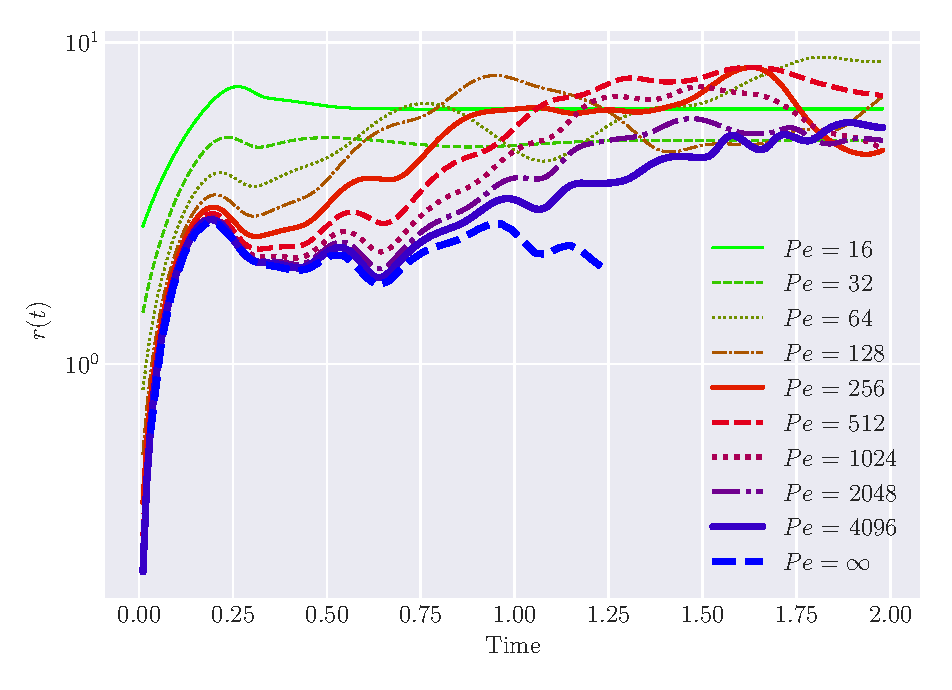
\includegraphics[width=0.5\textwidth]{enstrophy_rate}
\caption{Enstrophy}
\end{figure}


\begin{figure}
\includegraphics[width=\textwidth]{energy_film}
\caption{Local-in-time optimization with energy constraint. Top filmstrip is for $Pe = 4096$ and the bottom filmstrip is $Pe=256$.}
\end{figure}

\begin{figure}
\includegraphics[width=\textwidth]{energy_norms}
\caption{Energy}
\end{figure}

\begin{figure}
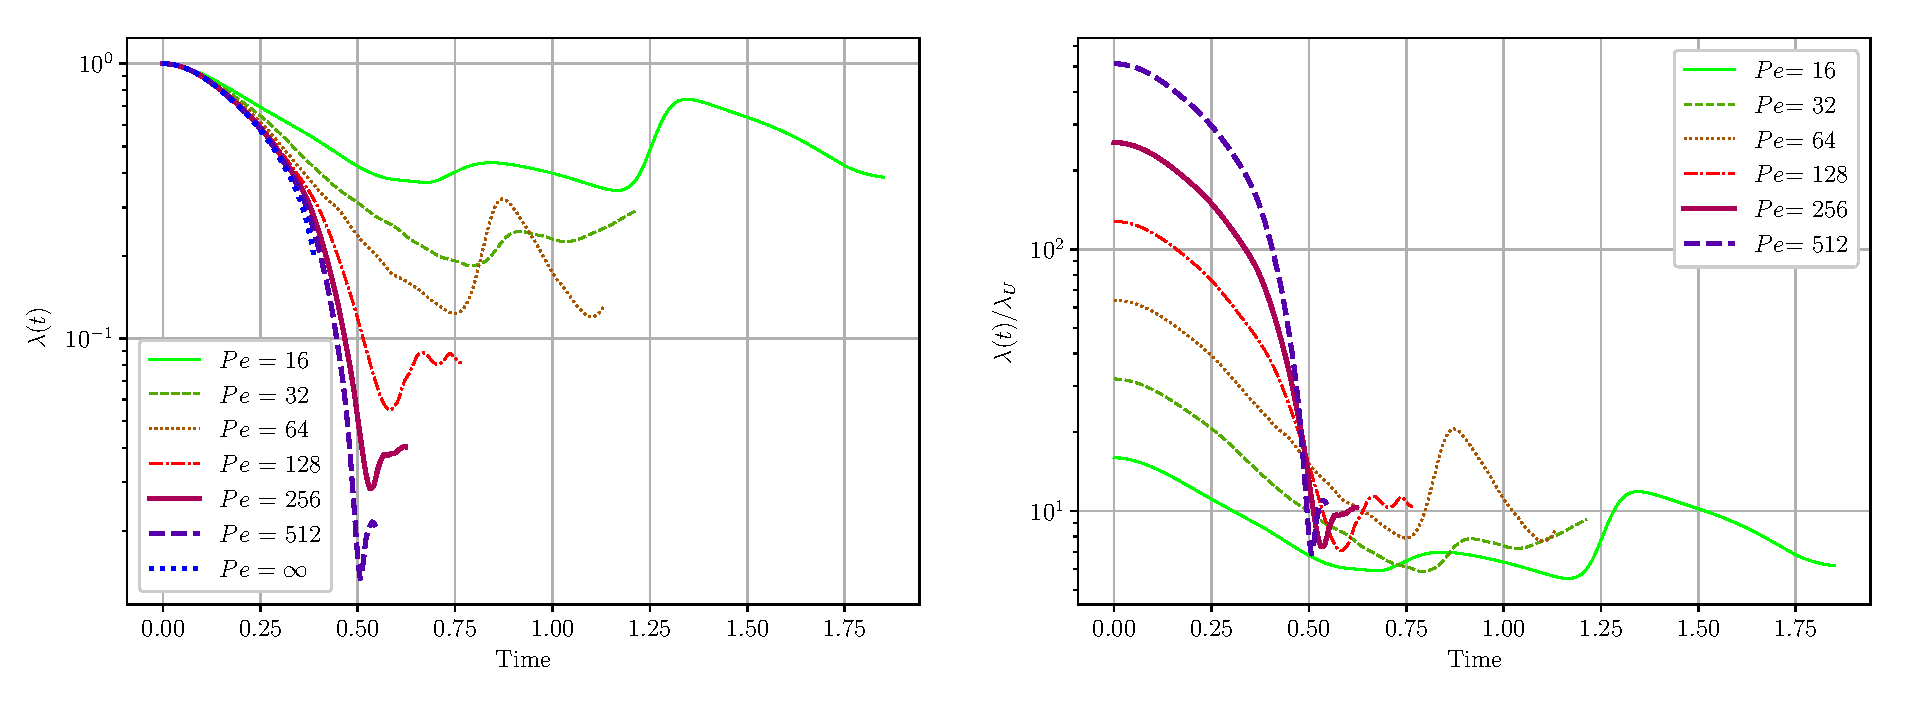
\includegraphics[width=\textwidth]{energy_length}
\caption{Energy}
\end{figure}

\begin{figure}
\centering
\includegraphics[width=\textwidth]{energy_rate}
\caption{Energy}
\end{figure}



%Define the spectral variance as
%%
%\begin{equation}
%		\left[ 
%			\frac{\hone{\theta}^2\hmone{\theta}^2}
%			{\ltwo{\theta}^4}  
%			- 1
%		\right].
%\end{equation}
%%
%By using this definition with H\"older's inequality provided that  $\linf{\nabla\vec{u}}\leq \Gamma$, we find that
%%
%\begin{equation}
%\label{eq:length_ineq_rate-of-strain}
%	\ddt{\lambda^2} \geq 2 1/Pe \sigma^2 - 2 \Gamma \lambda^2 .
%\end{equation}
%%
%By taking the long-time average (noted as $\langle \cdot \rangle \equiv\lim_{T\rightarrow\infty}\frac{1}{T}\int_{0}^T \,\, \cdot \,\, dt $ ) of the inequality above, we find that 
%%
%\begin{equation}
%	0 \geq  2 \kappa \tavg{\sigma^2} - 2 \Gamma \tavg{\lambda^2}.
%\end{equation}
%%
%The left hand side is zero since $\lambda^2$ is bounded by Poincar\'e's inequality. Thus, we find that
%%
%\begin{equation}
%	\tavg{\lambda^2} \geq   \lambda_{B}^2 \tavg{\sigma^2} 
%\end{equation}
%%
%where the Batchelor scale is given by $\lambda_{B} = \sqrt{\kappa/\Gamma}.$ 



\section{Conclusion}

We conclude that ...

\
\section*{Acknowledgements}

We thank ....

\appendix
\section{Numerical analysis}
\label{sec:num_analysis}
\bibliographystyle{jfm}
%% Note the spaces between the initials
\bibliography{manuscript}

\end{document}
